\documentclass[13pt, letterpaper, oneside]{book}
\usepackage{graphicx}

\usepackage[driver=xetex,paperwidth=8.5in,paperheight=11in,left=1.2in,
right=1in,top=1.3in, bottom=1.4in]{geometry}
\usepackage[no-math]{fontspec}
\usepackage{newfloat}
\usepackage{sectsty, tikz, color, pgfplots}
\usetikzlibrary{shapes,arrows}
\usepackage{multicol}
\usepackage{amsmath, amssymb, amsfonts,  titlesec}
\usepackage[urw-garamond,cal=cmcal]{mathdesign}
\usepackage{fancyhdr, booktabs, longtable}
%\usepackage[font=small,format=plain,labelfont=it,textfont=it]{caption}
\usepackage{caption,subcaption}
\usepackage{listings}
\usepackage{algpseudocode, algorithm,setspace}
% \usepackage[T1]{fontenc} 
\usepackage{enumitem,verbatim,natbib}

 \DeclareTextCommandDefault{\nobreakspace}{\leavevmode\nobreak\ } 

%========== DEFINITIONS ==========

\newlist{alist}{itemize}{1}
\setlist[alist]{label=--,labelindent=2in,leftmargin=9pt,labelsep=6pt, itemsep=0pt}

\def\Lmax{L_{\text{max}}}
\def\est{\mathtt{est}}
\def\lst{\mathtt{lst}}
\def\eft{\mathtt{eft}}
\def\lft{\mathtt{lft}}
\def\startOf{\mathtt{startOf}}
\def\endOf{\mathtt{endOf}}

%=========== TIKZ STUFF =========

\usetikzlibrary{fit}
\makeatletter
\tikzset{
  fn/.style={
    inner sep=0pt,
    fill=none,
    draw=none,
    reset transform,
    fit={(\pgf@pathminx,\pgf@pathminy) (\pgf@pathmaxx,\pgf@pathmaxy)},
  },
  reset transform/.code={\pgftransformreset}
}
\makeatother

%========= ALGO STUFF ============

%========= FONT SPECS ============
\tolerance 8000

\defaultfontfeatures{Mapping=tex-text, Ligatures=Common}

%\renewcommand\refname{references} % this sets the name of
\def\labelitemi{--}

\def\sansfont{\fontspec[Script=Latin,LetterSpace=2.6, Mapping=tex-text]{DIN 1451 Mittelschrift}}
\def\sansitalicfont{\fontspec[Script=Latin,LetterSpace=2.6, FakeSlant=0.2, Mapping=tex-text]{DIN 1451 Mittelschrift}}

\def\monofont{\fontspec[Script=Latin,Mapping=tex-text,Scale=0.91, AutoFakeBold]{Inconsolata}}

\renewcommand{\texttt}[1]{{\monofont #1}}
\renewcommand{\mathtt}[1]{{\text{\monofont #1}}\,}

\renewcommand{\normalsize}{\fontsize{12pt}{16pt}\selectfont}

%========== COLOR STUFF ===============

\definecolor{darkred}{rgb}{0.6, 0, 0.00}


%============ LISTINGS ==============
\lstset{
aboveskip=2\medskipamount, belowskip=2\medskipamount,
basicstyle=\monofont,
language=python,
numbers=left, numberstyle=\tiny,  numbersep=9pt,
xleftmargin=.4in, frame=l, xrightmargin=1.74in
}


%============= PAGE LAYOUT ============

%\titleformat{\section}{\huge\sansnormalfont}{\protect\makebox[0pt][r]{\thesection\quad}}{0em}{}
\titleformat{\chapter}{\fontsize{32pt}{36pt}\selectfont\sansfont}{}{0em}{}
\titleformat{\section}{\fontsize{18pt}{22pt}\selectfont\sansfont}{\protect\makebox[0pt][r]{\thesection\quad}}{0em}{}
\titleformat{\subsection}{\fontsize{12pt}{16pt}\selectfont\sansfont}{\protect\makebox[0pt][r]{\thesubsection\fontsize{18pt}{22pt}\selectfont\quad}}{0em}{}
%\titleformat{\paragraph}{\fontsize{12pt}{16pt}\selectfont}{}{}{}


\fancyhead[LE]{\sansfont\small Scheduling non-identical jobs on a batch resource \normalsize}
\fancyhead[RE]{}
\fancyhead[LO]{}
\fancyhead[RO]{\sansfont\small \nouppercase\rightmark}
\fancyfoot[C]{\sansfont\thepage}

\fancypagestyle{plain}{
\fancyhf{}
\renewcommand{\headrulewidth}{0pt}
\fancyfoot[C]{\sansfont\thepage}
}

%====== CHAR REPLACEMENTS ======%
\let\oldemptyset\emptyset
\let\emptyset\varnothing

%===== LONG EQUATION THINGS =====%
\DeclareFloatingEnvironment[
  fileext=los,
  listname=List of Models,
  name=Model,
  placement=tbhp,
  within=section
]{model}



\usepackage[hidelinks]{hyperref}

\begin{document}
%\begin{comment}
\frontmatter

\fontsize{12pt}{16pt}\selectfont
\thispagestyle{empty}
\pagestyle{fancy}

\baselineskip=16.8pt plus 0pt
\frenchspacing

\begin{centering}
\vspace{3em}
\LARGE\sansfont{Scheduling non-identical jobs on a batch resource}

\vspace{2em}
\large
\sansfont Sebastian Kosch\\

\vfill
\normalfont
\fontsize{12pt}{16pt}\selectfont
A thesis submitted in conformity with the requirements

for the degree of \textit{Bachelor of Applied Science}

\vspace{1em}
Supervisor: Prof. J. Christopher Beck, MIE

\vspace{2em}

\textmd Division of Engineering Science\\
University of Toronto\\

April 2013

\end{centering}
\pagebreak

%\include{firstpage}

\tableofcontents
\listoffigures
\listoftables
%\end{comment}
\pagestyle{fancy}
\mainmatter
\pagebreak
\vskip 4em
\fontsize{12pt}{17pt}\selectfont
\chapter{Introduction}
This paper discusses three different approaches, and several variations on them,
to solving the problem of scheduling non-identical jobs on a batch processing
machine. Batch processing machines, for the purposes of this paper, can process
multiple, non-identical jobs simultaneously---but all jobs must be loaded into
and unloaded from the machine at once, which introduces a considerable twist on
the ``simple parallel resources'' known from typical example problems in
existing literature.

The machines in question represents real-life resources like autoclaves or
ovens, which can process multiple items at a time, but often cannot be opened at
random---in fact, such machines often need to wait for the largest item in the
batch to be done before the next batch can be inserted.

\citet{Malapert} proposed a global constraint programming algorithm consisting
of a set of filtering rules to solve the problem. He achieved considerably
better speeds than with a simple mixed-integer model, but it seems plausible
that the new global constraint is unnecessary to achieve this performance;
simple MIP, CP or decomposition approaches are easier to implement and extend.
In this paper, we present 1) an improvement to his MIP model, 2) a CP model and
3) a decomposition approach to ``divide and conquer'' the problem.

\section{Problem definition}
We describe the problem as follows: assume we are given a set of jobs $J$, each of
which has a processing time (or ``length'') $p_j$ and a size (or ``capacity
requirement'') $s_j$. Each job also
has a due date $d_j$. The machine is characterized by its capacity $b$, and in
every batch, the jobs' summed sizes must not exceed this number. All values are
integer.

The machine can only process one batch $k$ of jobs at a time, and batches always
take as long as the longest job in the batch (i.e. $P_k = \max_{j \in k}(p_j)$).
Our objective is to minimize the lateness $L$ of the latest job in $J$, where
$L$ is the difference between the job's completion time $C_j$ and its due date
$d_j$---in formal terms, \textit{min.} $\Lmax = \max_j(C_j - d_j)$. The job's
completion time, however, is the completion time of the batch, which in turn
finishes with its \textit{longest} job as stated above.

Malapert uses the standard format established by Graham et al. to
summarize the problem as $1|\textit{p-batch}; b < n;
\textit{non-identical}|\Lmax$, where $\textit{p-batch};b<n$ represents the
parallel-batch nature and the finite capacity of the resource. A simpler version
with identical job sizes was shown to be strongly NP-hard in \citep{Brucker};
this problem, then, is no less difficult.

It helps to visualize the jobs before delving into the technicalities of
scheduling them. Figure \ref{fig:intro_tetris} shows a solution to a sample
problem with eight jobs and a resource with capacity $b = 20$.

\begin{figure}
  \centering
    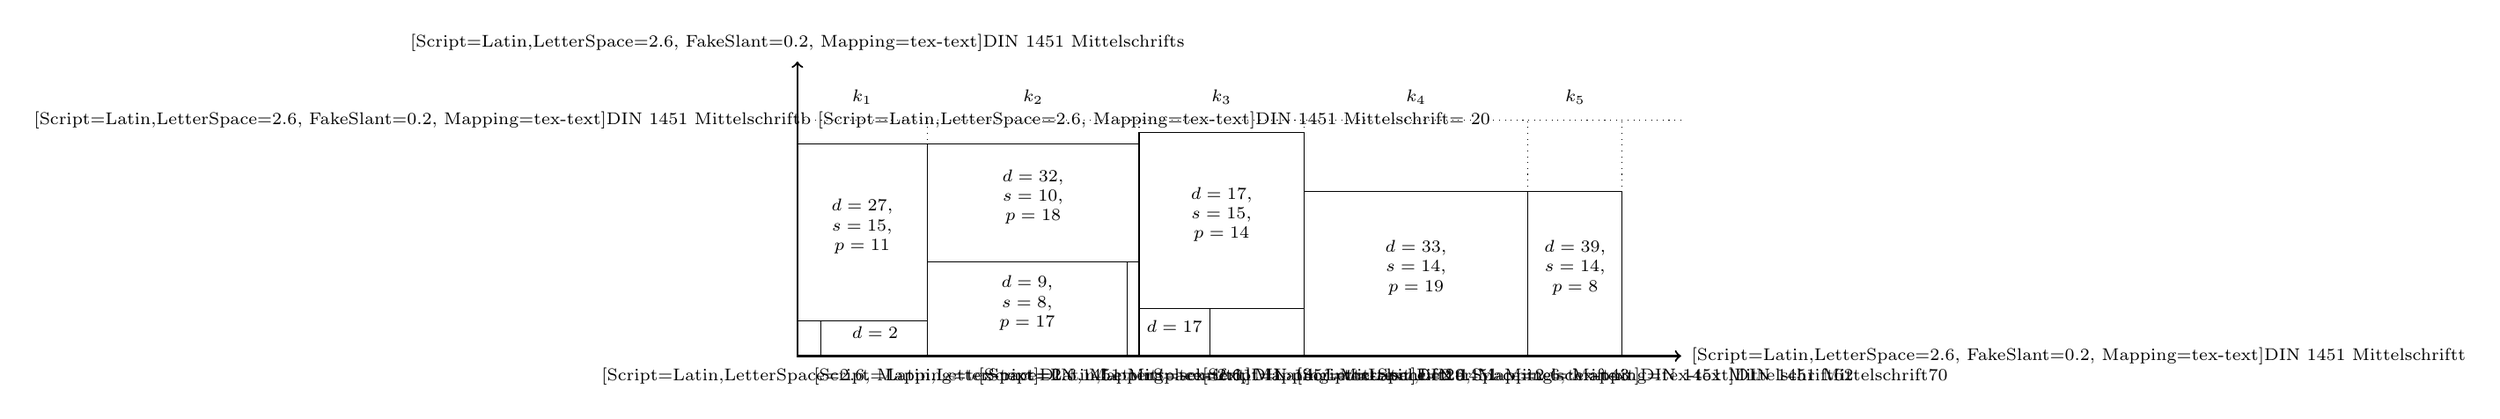
\begin{tikzpicture}[scale=0.17, font=\scriptsize]
      \draw [<->,thick] (0,25) node (yaxis) [above] {\sansitalicfont s}
        |- (75,0) node (xaxis) [right] {\sansitalicfont t};
      \draw[dotted] (0,20) -- (75,20);
      \node at (-3, 20) {{\sansitalicfont b }\sansfont = 20};
        \draw (0,0) rectangle (2,3) node[fn, xshift=2.3em, text width=4em] {$d = 2$};
        \draw (0,3) rectangle (11, 18) node[fn] {$d = 27,$\\ $s=15,$\\ $p = 11$};
        \node at (5.5, 22) {$k_1$};
        \node at (11, -1.7) {\sansfont 11};
      \draw[dotted] (11,0) -- (11,20); 
        \draw (11,0) rectangle (28, 8) node[fn] {$d = 9,$\\ $s=8,$\\ $p=17$};
        \draw (11,8) rectangle (29,18) node[fn] {$d = 32,$\\ $s=10,$\\ $p=18$};
        \node at (20, 22) {$k_2$};
        \node at (29, -1.7) {\sansfont 29};
      \draw[dotted] (29,0) -- (29, 20);
        \draw (29,0) rectangle (35,4) node[fn] {$d = 17$};
        \draw (29,4) rectangle (43,19) node[fn] {$d = 17,$\\ $s=15,$\\ $p=14$};
        \node at (36, 22) {$k_3$};
        \node at (43, -1.7) {\sansfont 43};
      \draw[dotted] (43,0) -- (43, 20);

        \draw (43,0) rectangle (62, 14) node[fn] {$d = 33,$\\ $s=14,$\\ $p=19$};
         \node at (52.5, 22) {$k_4$};
        \node at (62, -1.7) {\sansfont 62};

      \draw[dotted] (62,0) -- (62, 20);
        \draw (62,0) rectangle (70, 14) node[fn] (lastblock) {$d = 39,$\\
        $s=14,$\\ $p=8$};
         \node at (66, 22) {$k_5$};
        \node at (70, -1.7) {\sansfont 70};
      \draw[dotted] (70,0) -- (70, 20);

    \end{tikzpicture}
 \caption{Optimal solution to an example problem with eight
 jobs ($s_j$ and $p_j$ not shown for the two small jobs)}\label{fig:intro_tetris}
\end{figure}

\section{Organization of this paper}
After reviewing some of the most relevant publications on both general MIP/CP models and
batch scheduling problems, we first describe Malapert's original MIP model in
section \ref{sec:malapertmipmodel}. We then present possible improvements to the
model in \ref{sec:improvedmipmodel}. Section \ref{sec:cpmodel} introduces a CP formulation of the same
problem. Sections \ref{sec:mipdecomp} and \ref{sec:cpdecomp} describe a
decomposition approach.

An empirical comparison of the new models and a discussion of the results follow in
sections \ref{sec:results} and \ref{sec:discussion}. Ideas for future work are
listed in \ref{sec:futurework}.

\chapter{Background}
% citet{Azizoglu} results in [2002]
% citep{Azizoglu} results in [Azizoglu et al., 2002]
% citep*{Azizoglu} results in [Azizoglu and Miller, 2002]
Many optimization problems, and scheduling problems in particular, are
combinatorial in nature. The number of possible solutions grows exponentially
with the number of input variables, and even with fast computers it is
impossible to explore all of them individually to find the best one
(also called ``full enumeration'', or ``brute-force'' search) in a reasonable
amount of time. Often, however, it is possible to reason about subsets of
solutions that are known to be suboptimal a priori. This limits the search
space, allowing us to solve many instances of difficult combinatorial problems
in few hours, minutes or even seconds.

Such constrained searches are often implemented in either of two ways (or
variants of them): as a \textit{Constraint Programming model} (CP) or as a
\textit{Mixed Integer Programming model} (MIP). In this section I will briefly
introduce the concepts behind both CP and MIP and review recent work on problems
similar to the one dealt with here.

\section{Algorithmic concepts}
\subsection{Constraint Programming}
A constraint program specifies relationships, \textit{constraints}, that must
hold between input variables in the form of mathematical equations or
inequalities. Every input variable is assigned a set $\mathcal{D}$ of potential
values it can assume, its \textit{domain}. The solving algorithm begins by
assigning a value to one of the variables. Using the constraints, the solver can
then often reduce the other variables' domains, i.e. eliminate other potential
values of other variables. These domain reductions may themselves trigger domain
reductions in other variables, and so on, in a process called
\textit{propagation}. Propagation can lead to one of three results:
\begin{alist}
\item{an inconsistency, in which a variable's domain is reduced to an empty set.
That is, the given constraints allow for none of that variable's
potential values given the values assigned to other variables. As a result, the
solver will \textit{backtrack}, i.e. undo one or more of previous assignments
made, and assign other values.}
\item{a consistent solution, in which every variable's domain is reduced to a single value
(a singleton). If we are searching for an optimal solution, this may replace an
incumbent solution if it is better.}
\item{some reduced domains, but neither a solution nor an inconsistency. In this
case, the solver assigns more values to variables to trigger more propagation,
until a solution or an inconsistency is reached.}
\end{alist}

Without formally introducing different notions of inconsistency, it should be
noted that a problem can have no solution even when all variables have
non-empty domains. (See figure).

Unlike in MIP, constraints in CP are not restricted to expressions that are
linear in the input variables. Furthermore, so-called \textit{global
constraints} can be used that act on entire sets of variables at once. They are
implemented as custom algorithms that rely on specific knowledge about the
problem and are often based on results from graph theory. Global constraints can
be powerful tools; a classic example is the \texttt{alldifferent} constraint
which ensures that a set of variables take on unique values. While a number of
not-equal relationships between the variables can achieve the same effect after
several propagations, the global constraint reduces the domains of all involved
variables in one fell swoop such that for each variable, only the values remain
that are consistent with those of all the other variables.

\subsection{Mixed Integer Programming}
Similar to CP searches, MIP searches can be thought of as trees, where every
branch represents an assignment of a value to a domain and every leaf represents
a feasible solution. The difference lies in the way MIP explores this search tree.

MIP models are Linear Programming models (LPs) in which some of the decision
variables are declared integers--thus the name, and thus the restriction to
linear constraints. Like LP models, MIP models also require an objection
function to be minimized. The MIP solver first solves the problem as an LP,
which generally results in fractional values for most variables, such as $x =
a$. It then branches on possible values for $x$: either $x < a$ or $x > a$. If
$a$ is integral, $x = a$.  The MIP solution at a node $n$ also serves as a
\textit{lower bound} $LB_n$ on solutions in the respective subtrees: once a
solution with an objective value of $v$ is found, $v$ becomes an \textit{upper
bound} on the optimal objective value and all yet unexplored subtrees with $LB_n
\geq v$ need no longer be searched (``pruning'' the subtree). This procedure is
called \textit{branch-and-bound} and the most basic method used to solve integer
programming problems. Other methods exist, e.g. \textit{branch-and-cut}, and are
often used in conjunction with branch-and-bound in today's solvers.

\section{Literature}
The problem at hand is based on the work of \citet{Malapert}, who proposed a global
constraint \texttt{sequenceEDD} to be used in combination with \texttt{pack} to
solve it to optimality. The \texttt{sequenceEDD} constraint is implemented as
four distinct filtering rules applied at relevant domain changes: three to update
bounds on $\Lmax$ based on different conditions, and one to limit the number of
batches based on the marginal cost difference between adding a job to an empty batch vs. an
existing one. The new global was shown to significantly outperform a simple MIP model of the same problem.

Other authors have examined similar problems: \citet{Azizoglu} provide an exact
method and a heuristic for the same problem, but minimize makespan
($C_\text{max}$) instead of $\Lmax$, as have \cite{Dupont}. Similar exact
methods have been proposed for multi-agent variants with different objective
functions \citep{Sabouni}, for makespan minimization on single batch machines
\citep{Kashan}, and for makespan minimization on parallel batch machines with
different release dates \citep{Ozturk}. A more extensive review of MIP model
applications in batch processing is given by \citet{Grossmann}.

\chapter{Modelling the problem}

\section{MIP model}
Malapert's original MIP approach, as given in Model \ref{model:malapertmip},
uses a set of binary decision variables $x_{jk}$ to represent whether job $j$ is
assigned to batch $k$. The original model assumes a set $K$ of $|K| = |J|$
batches, the number of jobs being a trivial upper bound on the number of
batches required; it also enforces an earliest-due-date-first (EDD) ordering of
the batches (constraint \ref{c:malapp-edd}).
\begin{model}[h]
\begin{alignat}{2}
\mathrm{Min.}\quad & \Lmax && \\
\mathrm{s.t.}\quad &\sum_{k \in K} x_{jk} = 1 \quad && \forall j \in J \\
  &\sum_{j \in J} s_j x_{jk} \leq b \quad && \forall k \in K\\
  &p_j x_{jk} \leq P_k \quad && \forall j \in J, \forall k \in K\\
  &C_{k-1} + P_{k} = C_k \quad && \forall k \in K\\
  &(d_{max} - d_j)(1 - x_{jk}) + d_j \geq D_k \quad && \forall j \in J, \forall k \in K\\
  &D_{k-1} \leq D_k \quad && \forall k \in K \label{c:malapp-edd} \\
  &C_k - D_k \leq \Lmax \quad && \forall k \in K\\[2ex]
  &C_k \geq 0, P_k \geq 0 \text{ and } D_k \geq 0 \quad && \forall k \in K  
\end{alignat}
\caption{Malapert's original MIP model}
\label{model:malapertmip}
\end{model}

\section{Improved MIP model}
\subsection{Grouping empty batches}
The given formulation lacks a rule that ensures that no empty batch is followed by a non-empty batch. Empty batches have no processing time and a due date only bounded by $d_\text{max}$, so they can be sequenced between non-empty batches without negatively affecting $\Lmax$. Since, however, desirable schedules have no empty batches scattered throughout, we can easily reduce the search space by disallowing such arrangements. The idea is illustrated in Figure \ref{fig:dominancerule}.


\begin{figure}
  \centering
  \begin{subfigure}[b]{0.4\textwidth}
    \centering
    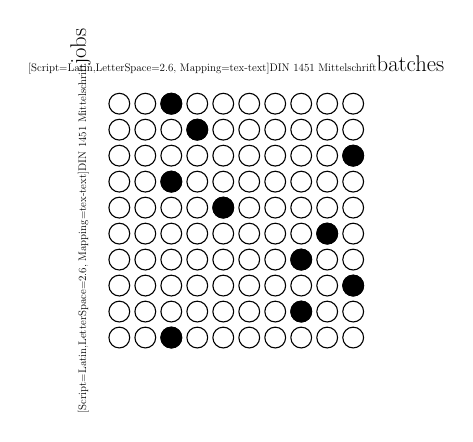
\begin{tikzpicture}[scale=0.33]
      \pgftext[x=-1.5cm, y=4.5cm, rotate=90]{\sansfont\Huge jobs}
      \pgftext[x=4.5cm, y=10.5cm]{\sansfont\Huge batches}

      \foreach \j in {0,...,9}
      {
        \foreach \k in {0,...,9}
        {
          \draw[] (\k, \j) circle [radius=0.4];
        }
      }
      \draw [fill] (2,0) circle [radius=0.4];
      \draw [fill] (2,6) circle [radius=0.4];
      \draw [fill] (2,9) circle [radius=0.4];
      \draw [fill] (3,8) circle [radius=0.4];
      \draw [fill] (4,5) circle [radius=0.4];
      \draw [fill] (7,1) circle [radius=0.4];
      \draw [fill] (7,3) circle [radius=0.4];
      \draw [fill] (8,4) circle [radius=0.4];
      \draw [fill] (9,2) circle [radius=0.4];
      \draw [fill] (9,7) circle [radius=0.4];
    \end{tikzpicture}
    \caption{Without dominance rule}
  \end{subfigure}
  \begin{subfigure}[b]{0.4\textwidth}
    \centering
    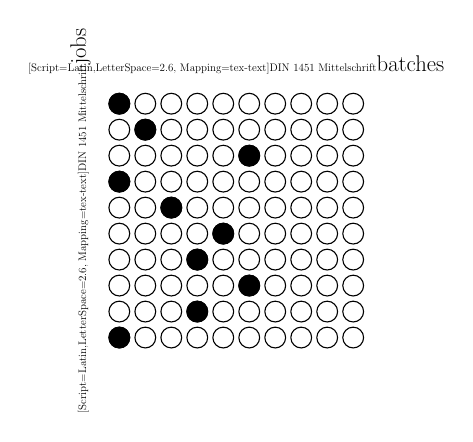
\begin{tikzpicture}[scale=0.33]
      \pgftext[x=-1.5cm, y=4.5cm, rotate=90]{\sansfont\Huge jobs}
      \pgftext[x=4.5cm, y=10.5cm]{\sansfont\Huge batches}

      \foreach \j in {0,...,9}
      {
        \foreach \k in {0,...,9}
        {
          \draw[] (\k, \j) circle [radius=0.4];
        }
      }
      \draw [fill] (0,0) circle [radius=0.4];
      \draw [fill] (0,6) circle [radius=0.4];
      \draw [fill] (0,9) circle [radius=0.4];
      \draw [fill] (1,8) circle [radius=0.4];
      \draw [fill] (2,5) circle [radius=0.4];
      \draw [fill] (3,1) circle [radius=0.4];
      \draw [fill] (3,3) circle [radius=0.4];
      \draw [fill] (4,4) circle [radius=0.4];
      \draw [fill] (5,2) circle [radius=0.4];
      \draw [fill] (5,7) circle [radius=0.4];
    \end{tikzpicture}
    \caption{With dominance rule}
  \end{subfigure}
\caption{Dominance rule to eliminate empty batches followed by non-empty batches
(circles represent the $x_{jk}$ variables; a filled circle stands for $x_{jk} =
1$)}\label{fig:dominancerule}
\end{figure}


A mathematical formulation is
\begin{alignat}{2}
& \sum_{j \in J} x_{j,k-1} = 0 \rightarrow \sum_{j \in J} x_{jk} = 0 \quad && \forall k \in K. \label{eq:emptybatch0}
\end{alignat}

To implement this, we can write constraints in terms of an additional  set of binary variables, $e_k$, indicating whether a batch $k$ is empty or not:

\begin{alignat}{2}
& e_k + \sum_{j \in J} x_{jk} \geq 1 \quad && \forall k \in K, \label{eq:emptybatch1} \\
& n_j (e_k-1) + \sum_{j \in J} x_{jk} \leq 0 \quad && \forall k \in K. \label{eq:emptybatch2}
\end{alignat}

Constraints \eqref{eq:emptybatch1} enforce $e_k = 1$ when the batch $k$ is
empty. Constraints \eqref{eq:emptybatch2} enforce $e_k = 0$ otherwise, since the sum term will never exceed $n_j$. The rule \ref{eq:emptybatch0} can now be expressed as $e_{k-1} = 1 \rightarrow e_k = 1$, and implemented as follows:

\begin{alignat}{2}
& e_k - e_{k-1} \geq 0 \quad && \forall k \in K.
\end{alignat}

We can also prune any attempts to leave the first batch empty by adding a constraint $e_0 = 0$.

{\color{darkred} This, while it works just fine, actually takes longer than without it.}

\subsection{No postponing of jobs to later batches}
Since the jobs are already sorted by non-decreasing due dates, it makes sense to explicitly instruct the solver never to attempt to push jobs into batches with a greater index than their own: even if every job had its own batch, it would be unreasonable to ever postpone a job to a later batch.
\begin{alignat}{2}
  & x_{jk} = 0 \quad && \forall \{j \in J, k \in K | j > k \}
\end{alignat}




\section{CP model}
The constraint programming model is based on a set of decision variables $B_j =
\{k_1, \dots, k_{n_k} \}$, where each variable stands for the batch job $j$ is
assigned to. The complete model is given in Model \ref{model:cpmodel}.

\begin{model}

\begin{alignat}{2}
\mathrm{Min.}\quad & \Lmax && \\
\mathrm{s.t.}\quad & \label{cpcs:pack} \mathtt{pack}(J, K, b) && \\
& \label{cpcs:cumul} \mathtt{cumul}(J, b) && \\
& \label{cpcs:pk} P_k = \underset{j}{\max} \; p_j \quad && \forall \{j \in J
| B_j = k\}, \forall k \in K \\
& \label{cpcs:dk} D_k = \underset{j}{\min} \; d_j \quad && \forall \{j \in J
| B_j = k\}, \forall k \in K \\
& \label{cpcs:ck} C_k + P_{k+1} = C_{k+1} \quad && \forall k \in K \\
& \label{cpcs:lmax} \Lmax \geq \underset{k}{\max} \; (C_k - D_k) && \\
& \label{cpcs:empty} \mathtt{IfThen}(P_k = 0, P_{k+1} = 0) \quad && \forall k
\in \{ k_1, \dots, k_{n_k - 2}\} \\
& \label{cpcs:pp} B_j \leq k \quad && \forall \{ j \in J, k \in K | j > k \}
\end{alignat}
\caption{Constraint programming model}
\label{model:cpmodel}
\end{model}

Constraint \eqref{cpcs:pack} makes sure the jobs are distributed into the
batches such that no batch exceeds the capacity $b$. Constraint
\eqref{cpcs:cumul}, a global cumulative constraint, keeps jobs from overlapping
on the resource -- while redundant with \eqref{cpcs:pack}, this speeds up
propagation slightly. Constraints \eqref{cpcs:pk}, \eqref{cpcs:dk},
\eqref{cpcs:ck} and \eqref{cpcs:lmax} define $P_k$, $D_k$, $C_k$ (batch
completion time) and $\Lmax$, respectively.



\subsection{Temporal constraints on a job's start date} Given any partial
assignment of jobs and an open job $j$, we can reason that \begin{alist}
\item{if the first batch with a due date later than the job is $k$, then the job
cannot be part of a batch after $k$ -- this would result in a non-EDD sequence
of batches.} \item{if the first batches up to $k-1$ offer not enough capacity
for $j$ due to the given partial assignment, then the job cannot be part of a
batch before $k$.} \end{alist} Since batches are \textit{not} dynamically
created like in Malapert's solution but fixed from the start, any partial
assignment that fails due to these constraints cannot be part of an optimal
solution.

This constraint is redundant with both the $(C_{k+1}\geq C_k)$ and
\texttt{packing} constraints, but may help accelerate the propagation in some
cases.

\subsection{Grouping empty batches} Just like in the MIP model, we can force
empty batches to the back and thus establish dominance of certain solutions. The
implementation is much easier than in the MIP model: \begin{alignat}{2} &
\mathtt{IfThen}( C_{k+2} > C_{k}, C_{k+1} > C_{k} ) \quad && \forall k \in
\{k_1, \dots, k_{n_k-2}\} \end{alignat}

\subsection{No postponing of jobs to later batches} Just like in the MIP model,
jobs should never go into a batch with an index greater than their own:
\begin{alignat}{2} & x_{jk} = 0 \quad && \forall j,k : j > k \end{alignat} This
is implemented as $\mathtt{assignments}_j \leq k$. 

{\color{darkred} This constraint is analogous to the concept of finding an upper
bound on $n_k$ -- essentially, it would be very helpful to find an upper bound
on the latest batch for \textit{every} job.}



\section{Decomposition approach}

Instead of solving the entire problem using one model, we can solve the problem
step by step, using the best techiques available for each subproblem. This
approach is inspired by a method called \textit{Benders decomposition}.

\subsection{Branch-and-bound by batch in chronological order}
A basic version of this approach uses branch-and-bound to transverse the search
tree. At each node on level $\ell$, a single MIP and/or CP model is run to
assign jobs to batch $k = \ell$. The remaining jobs are passed to the children
nodes, which assign jobs to the next batch, and so on -- until a solution, and
thus a new upper bound on $\Lmax$, is found. Several constraints are used to
prune parts of the search tree that are known to offer only solutions worse than
this upper bound. Figure \ref{fig:decomp_diagram1} shows an example in which a
MIP model is used to assign jobs to the batch at every node.
\begin{algorithm}[h]
\fontsize{9pt}{11.5pt}\selectfont
\begin{algorithmic}
\State update \textit{currentAssignments} \Comment{this keeps track of where we are
in the tree}
\If{no jobs given to this node} \Comment{if this is a leaf node, i.e. all jobs
are assigned to batches}
  \State calculate $L_{\text{max,current}}$ based on \textit{currentAssignments}
  \If{$L_{\text{max,current}}$ < $L_{\text{max,incumbent}}$}
    \State $L_{\text{max,incumbent}} \gets L_{\text{max,current}}$
    \State \textit{bestAssignments} $\gets$ \textit{currentAssignments}
  \EndIf
  \State return to parent node
\EndIf
\State set up MIP model \Comment{as described below}
\Repeat
  \State $x_j \gets$ model.solve($x_j$) \Comment{let model assign jobs to the
  batch}
  \State spawn and run child node with all $\{j | x_j = 0\}$ \Comment{pass
  unassigned jobs to children}
  \State add constraint to keep this solution from recurring \Comment{this
  happens once the child node returns}
\Until{model has no more solutions}
\State return to parent node
\end{algorithmic}
\caption{MIP node class code overview}
\label{alg:bbnode_mip1}
\end{algorithm}
Algorithm \ref{alg:bbnode_mip1} outlines what happens at each node: the model
finds the best jobs to assign to the batch according to some rule, lets the
children handle the remaining jobs, and tries the next best solution once the
first child has explored its subtree and backtracked.
\subsubsection{Using MIP and cumulative packing after the batch}
\tikzset{
  treenode/.style = {align=center, inner sep=4pt, text centered,
    font=\sansfont\fontsize{11pt}{12pt}\selectfont},
  root/.style = {treenode},% arbre rouge noir, noeud noir
  nchild/.style = {treenode,
     },% arbre rouge noir, noeud rouge
  leaf/.style = {treenode}% arbre rouge noir, nil
}

\begin{figure}
\centering
\begin{tikzpicture}[->,>=stealth',level/.style={sibling distance = 3cm/#1,
  level distance = 1.5cm}, scale=0.7]
\node (Root) [root] {MIP}
 child{ node [nchild] {MIP} 
            child{ node [nchild] {MIP}}
            child{ node [nchild] {MIP}
              child{ node [leaf] {Solution 1}}
						}                            
    }
    child{ node [nchild] {MIP} }
    child{ node [nchild] {MIP} 
            child{ node [nchild] {MIP} %2, left
                    child{ node [leaf] {Solution 2}} 
                  }
            child{ node [nchild] {MIP} }
		};
  \begin{scope}[every node/.style={right}]
    \path (Root -| Root-3-2) ++(1.5cm,0) node {\fontsize{10pt}{10pt}\selectfont $k=1$};
    \path (Root-1 -| Root-3-2) ++(1.5cm,0) node
    {\fontsize{10pt}{10pt}\selectfont $k=2$};
    \path (Root-1-1 -| Root-3-2) ++(1.5cm,0) node
    {\fontsize{10pt}{10pt}\selectfont $k=3$};
  \end{scope}

   \end{tikzpicture}
\caption{Batch-by-batch decomposition using MIP only}\label{fig:decomp_diagram1}
\end{figure}

The first version of the branch-and-bound batch-by-batch decomposition uses a
MIP model at each node to assign jobs to the respective batch. The remaining
jobs are packed such as to minimize their $\Lmax$, with a relaxation of the
batching requirement, i.e., as if on a cumulative resource. 
\begin{model}[h!]
\begin{alignat}{3}
\text{Min.}\quad & L_{\text{max,cumul}} && \\ 
\text{s. t.}\quad & \label{dc:eq1} \sum_j s_j x_j \leq b \quad && \forall j \in J \\
& P_k \geq p_j x_j \quad && \forall j \in J \\
& \label{dc:eq3} \sum_j x_j \geq 1 \quad && \forall \{j \in J | d_j = \min(d_j)\} \\
& \label{dc:eq4} P_k + \frac{1}{b} \sum_{i} s_i p_i \leq d_j +
L_{\text{max,incmb}} - 1 - v_k \quad && \forall j \in J, \forall \{i \in J | d_i
\leq d_j\} \\[2ex]
& \label{dc:eq5} \sum_t u_{jt} = 1 \quad && \forall j \in J \\
& \label{dc:eq6} \sum_j \sum_{t' \in T_{jt}} s_j u_{jt'} \leq b \quad && \forall t \in \mathcal{H} \\
& \label{dc:eq7} (v_k + t + p_j) u_{jt} \leq d_j + L_{\text{max,incmb}} - 1 \quad && \forall j \in J, \forall t \in \mathcal{H} \\
& \label{dc:eq8} L_{\text{max,cumul}} \geq (v_k + t + p_j) u_{jt} - d_j \quad && \forall j \in J, \forall t \in \mathcal{H} \\
& \label{dc:eq9} u_{j,t=0} = x_j \quad && \forall j \in J \\
& \label{dc:eq10} u_{it} \leq (1 - x_j) \quad && \forall i,j \in J, \forall t
\in \{1, \dots, p_j - 1\} \\[2ex]
& \label{dc:eq11} b - \sum_{i \in J} s_i x_i \leq (b w_j + 1) s_j \quad && \forall j \in J \\
& \label{dc:eq12} P_k + 2w_j n_t \geq p_j + n_t x_j \quad && \forall j \in J\\
& \label{dc:eq13} P_k - 2(1 - w_j)n_t \leq p_j +n_t x_j - 1 \quad && \forall j
\in J
\end{alignat}
\caption{MIP model in batch-by-batch branch-and-bound}
\label{model:decomp_mip}
\end{model}

\begin{table}[h]
\begin{tabular}{l p{5in}}
$x_j$ & is 1 iff job $j$ is assigned to the batch \\
$u_{jt}$ & is 1 iff job $j$ starts in time slot $t$ \\
$T_{jt}$ & is the set of all time slots occupied by job $j$ if it ended at time
$t$, that is $T_{jt} = \{t - p_j + 1, \dots, t\}$ \\
$v_k$ & is the start time of the batch at the given node in the search tree \\
$L_{\text{max,incmb}}$ & is the incumbent (known best) value of and thus an
upper bound on $\Lmax$ \\
$\mathcal{H}$ & is the set of all indexed time points $\{0, \dots, n_t - 1\}$ \\
$w_j$ & is 1 iff job $j$ is either longer than the batch ($p_j > P_k$) or
already part of the batch ($x_j = 1$). Neither condition must be fulfilled for constraint
\eqref{dc:eq11} to have an effect on job $j$
\end{tabular}
\caption{Notation used in the decomposition model}
\end{table}

Model \ref{model:decomp_mip} implements a time-indexed cumulative constraint on the
non-batched jobs. Constraints \eqref{dc:eq1} through \eqref{dc:eq3} ensure that the
batch stays below capacity, define the duration of the batch $P_k$ and force at
least one of the earliest-due jobs into the batch.

Constraints \eqref{dc:eq4} express the interval relaxation used to ensure that no
jobs exceed their latest allowable finish date given any batch assignment. Even
jobs that are assigned to the batch have to fulfill this requirement.

Constraints \eqref{dc:eq5} and \eqref{dc:eq6} implement the cumulative nature of the
post-batch assignments by ensuring that each job starts only once, and no jobs
overlap on a given resource at any time.

Constraints \eqref{dc:eq7} again limit the possible end dates of a
job, but unlike \eqref{dc:eq4}, they use the time assignments on the cumulative
resource to determine end dates. Constraints \eqref{dc:eq8} define the value of
$L_{\text{max,cumul}}$, the maximum lateness of any job in the non-batched set.

Constraints \eqref{dc:eq9} force batched jobs to start at $t = 0$, while
\eqref{dc:eq10} force \textit{all} jobs to start either at $t = 0$ or after the
last batched job ends.

Constraints \eqref{dc:eq11} enforce a dominance rule: jobs must be assigned to
the batch such that the remaining capacity, $b_r = b - \sum_j s_j x_j$, is less
than the size $s_j$ of the \textit{smallest} job from the set of non-batched
jobs that are \textit{not longer} than the current batch. That is, if there
exists an non-batched job $j$ with $p_j \leq P_k$ and $s_j \leq b_r$, then the
current assignment of jobs is infeasible in the model. The reasoning goes as
follows: given any feasible schedule, assume there is a batch $k_a$ with $b_r$
remaining capacity and a later batch $k_b$ containing a job $j$ such that $s_j
\leq b_r$ and $p_j \leq P_{k_a}$. Then job $j$ can always be moved to batch
$k_a$ without negatively affecting the quality of the solution: if the schedule
was optimal, then moving $j$ will not affect $\Lmax$ at all (otherwise, it was
no optimal schedule); if the schedule was not optimal, then $\Lmax$ will stay
constant (unless $j$ was the longest job in $k_b$ and $\Lmax$ occured in or in a
batch after $k_b$, in which case $\Lmax$ will be improved).

This rule is implemented by means of a binary variable $w_j$, which, as defined
by constraints \eqref{dc:eq11} and \eqref{dc:eq12}, is 1 iff $p_j > P_k \lor x_j
= 1$. These are the cases in which a job $j$ is \textit{not} to be considered in
\eqref{dc:eq10}, and so $w_j$ is used to scale $s_j$ to a value insignificantly
large in the eyes of the constraint's less-than relation.

After a solution is found, a child node in the search tree has run the subtree
and returned, a constraint of the form 
\begin{alignat}{2}
& \sum_j x_j + \sum_i (1-x_i) \leq n_j - 1 \quad && \forall \{j \in J | x_j =
1\}, \forall \{i \in J | x_i = 0 \}
\end{alignat}\marginpar{\em\small I still can't think of anything tighter ...}
is added to the model before the solver is called again, to exclude the last
solution from the set of feasible solutions. 

\subsubsection{Using CP and cumulative packing after the batch}
This approach is equivalent, but we now use CP to select the batch assignments,
again based on a minimized $\Lmax$ among the non-batched jobs. Model
\ref{model:decomp_cp} uses interval variables $j$ to represent the jobs;
time constraints on the jobs (``est'', ``lft'' etc.) are represented as
equations involving the terms $\startOf(j)$ and $\endOf(j)$.

Contraints \eqref{dcp:eq1} through \eqref{dcp:eq4} bi-directionally define the
relationship between a job's $x_j$ and $\startOf(j)$: $x_j = 1$ is equivalent
with a start time of $t = 0$, and $x_j = 0$ is equivalent with a start time of
$t \geq P_k$. The term $\sum_{i \in J} p_i$ is used as a large constant as it is
greater than any job's start time.

Constraint \eqref{dcp:eq8} is equivalent to constraints \eqref{dc:eq11} through
\eqref{dc:eq13} in Model \ref{model:decomp_mip} above. The cumulative constraint
\eqref{dcp:eq9} ensures that jobs do not overlap. 

\begin{model}[h]
\begin{alignat}{2}
\mathrm{Min.} \quad & \Lmax \quad && \\
\mathrm{s.t.} \quad 
& \label{dcp:eq1} \startOf(j) \geq (1-x_j) P_k \quad && \forall j \in J \\
& \startOf(j) \leq (1-x_j) \sum_{i \in J} p_i \quad && \forall j \in J \\
& x_j \geq \frac{ \frac{1}{2} - \startOf(j) }{ \sum_{i \in J} p_i } \quad &&
\forall j \in J \\
& \label{dcp:eq4} x_j \leq 1+\frac{ \frac{1}{2} - \startOf(j)}{\sum_{i \in J} p_i } \quad &&
\forall j \in J \\
& P_k \geq \underset{j \in J}{\max}(x_j p_j) \quad && \\
& \endOf(j) = d_j + L_{\text{max,incmb}} - 1 \quad && \forall j \in J \\
& \Lmax \geq \endOf(j) - d_j \quad && \forall j \in J \\
& \label{dcp:eq8} \mathtt{IfThen}(p_j \leq P_k \land x_j = 0, b - \sum_{j \in J} s_j
x_j \leq s_j) \quad && \forall j \in J \\
& P_k + \frac{1}{b} \sum_i s_i p_i \leq d_j + L_{\text{max,incmb}} - 1 - v_k
\quad && \forall j \in J, \forall \{i \in J | d_i \leq d_j\} \\
& \sum_j x_j \geq 1 \quad && \forall \{ j \in J | d_j = \min(d_j) \} \\
& \label{dcp:eq9} \mathtt{cumul}(J, b) \quad & &  
\end{alignat}
\caption{CP model in batch-by-batch branch-and-bound}
\label{model:decomp_cp}
\end{model}





\newpage
\chapter{Results}
\section{Empirical comparison of described models}\label{sec:results}
The models were tested on a set of job lists. Malapert's paper uses benchmark
job lists by Daste et al. \cite{daste1, daste2}. Since neither publication is
available online, I created my own set of randomized job lists for the purposes
of this paper, with $s_j, p_j \in [1, 20]$ and $d_j \in [1, 10n_j]$ where $n_j$ is
the number of jobs. Ten different sample job sets are used per unique value of
$n_j$. The times shown in figure \ref{fig:comp_times} are averaged over those
ten instances for each $n_j$.

The \marginpar{\em\small I have not yet measured ``solution quality'' in any way
--- I suppose the number of batches required would be a good metric?} models were run on an i7 Q740 CPU in single-thread mode, with 8 GB RAM.
Solving was aborted after a time of 300 seconds (5 minutes).

The CP branch-and-bound model times out on most instances and is not shown here.
The CP model times out on one 12-job instance and gets progressively worse with
more jobs; similar to Malapert's original MIP model.
\begin{figure}
\centering

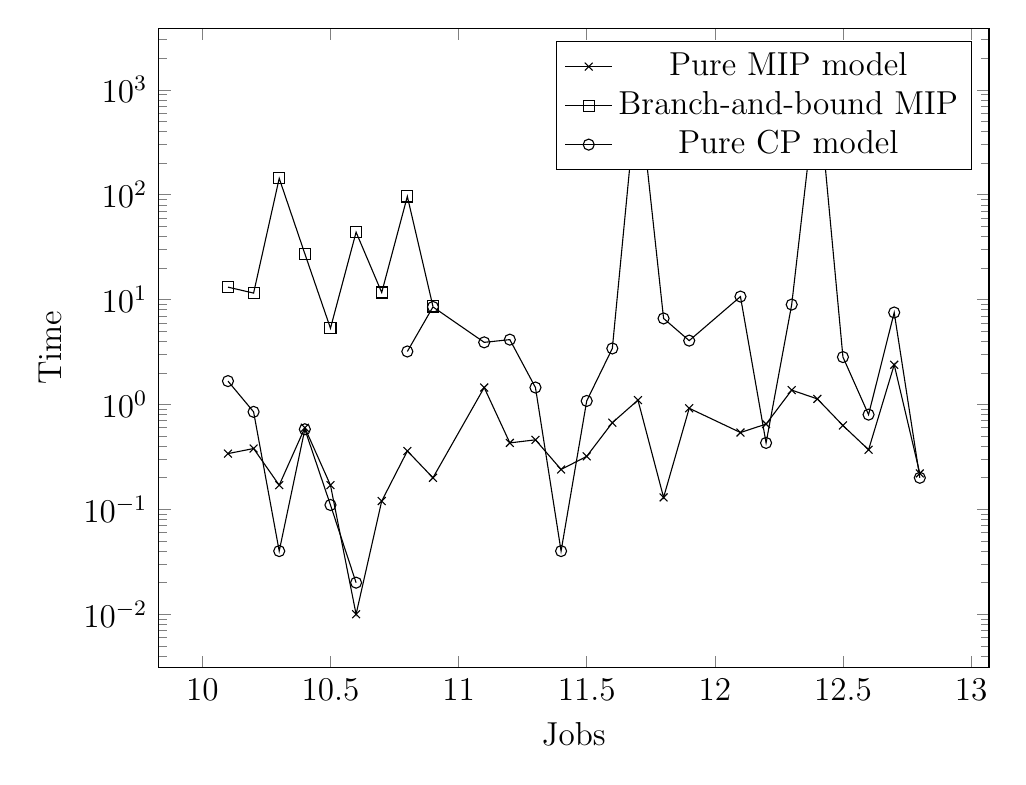
\begin{tikzpicture}
  \begin{semilogyaxis}[xlabel=Jobs, ylabel=Time, width=\textwidth,
  height=0.8\textwidth]
  \addplot[color=black, mark=x ] coordinates { % MIP model times
(10.1, 0.34)
(10.2, 0.38)
(10.3, 0.17)
(10.4, 0.6)
(10.5, 0.17)
(10.6, 0.01)
(10.7, 0.12)
(10.8, 0.36)
(10.9, 0.2)
(11.1, 1.45)
(11.2, 0.43)
(11.3, 0.46)
(11.4, 0.24)
(11.5, 0.32)
(11.6, 0.67)
(11.7, 1.1)
(11.8, 0.13)
(11.9, 0.92)
(12.1, 0.54)
(12.2, 0.65)
(12.3, 1.37)
(12.4, 1.13)
(12.5, 0.63)
(12.6, 0.37)
(12.7, 2.39)
(12.8, 0.22)
  };
  \addlegendentry{Pure MIP model}
  \addplot[color=black, mark=square] coordinates {
(10.1, 13.14)
(10.2, 11.53)
(10.3, 143.11)
(10.4, 27.34)
(10.5, 5.33)
(10.6, 43.9)
(10.7, 11.68)
(10.8, 96.27)
(10.9, 8.6)
  };
  \addlegendentry{Branch-and-bound MIP}
  \addplot[color=black, mark=o] coordinates {
(10.1, 1.67)
(10.2, 0.85)
(10.3, 0.04)
(10.4, 0.58)
(10.5, 0.11)
(10.6, 0.02)

(10.8, 3.2)
(10.9, 8.51)
(11.1, 3.91)
(11.2, 4.15)
(11.3, 1.45)
(11.4, 0.04)
(11.5, 1.08)
(11.6, 3.42)
(11.7, 1200)
(11.8, 6.61)
(11.9, 4.06)
(12.1, 10.68)
(12.2, 0.43)
(12.3, 8.96)
(12.4, 1200)
(12.5, 2.83)
(12.6, 0.8)
(12.7, 7.53)
(12.8, 0.2)
};
  \addlegendentry{Pure CP model}
  \end{semilogyaxis}
\end{tikzpicture}

\caption{Comparison of CPU time used by different models.}
\label{fig:comp_times}
\end{figure}





\chapter{Discussion}
The improved MIP model currently performs best.

\chapter{Unexplored ideas}
\section{MIP model}
\subsection[Upper bound on $\Lmax$]{Upper bound on {\sansitalicfont L}\textsubscript{max}}
An upper bound on $\Lmax$ can be found by using a dispatch rule to find a
feasible, if not optimal, schedule. A good approach could be the ``best-fit''
heuristic proposed in the original paper. {\color{darkred} This has not been
implemented yet.}

\subsection[Bounding the number of batches $n_k$]{Bounding the number of batches \sansitalicfont n\textsubscript{k}}
Initially, the number of batches needed is assumed to be equal to the number of
jobs: $n_k = n_j$. Reducing $n_k$ by pre-computing the maximum number of batches
needed shrinks the $x_{jk}$ matrix, and prunes potential search branches in
branch-and-bound decomposition approaches.


\begin{figure}
  \centering
  \begin{subfigure}[b]{0.4\textwidth}
    \centering
    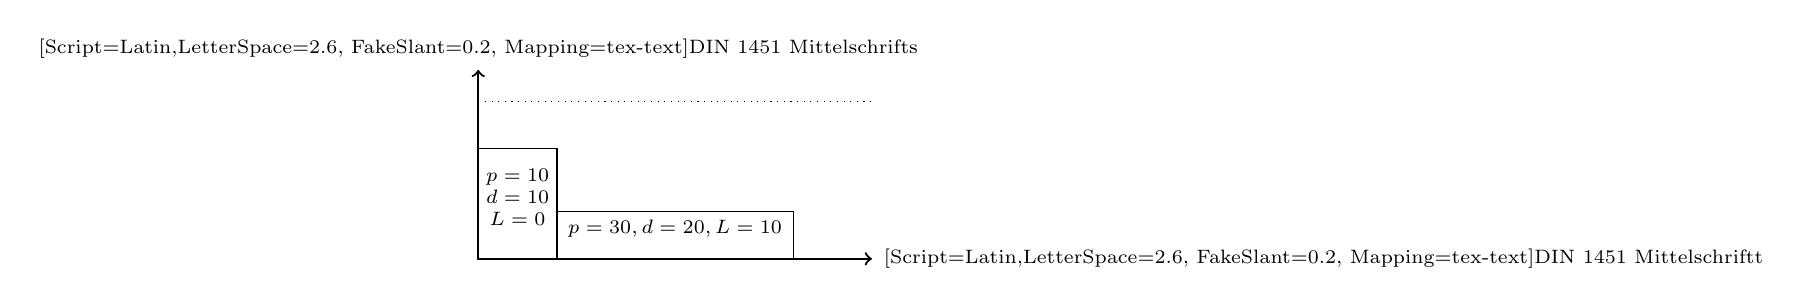
\begin{tikzpicture}[scale=0.2, font=\scriptsize]

      \draw [<->,thick] (0,12) node (yaxis) [above] {\sansitalicfont s}
        |- (25,0) node (xaxis) [right] {\sansitalicfont t};
      \draw[dotted] (0,10) -- (25,10);
        \draw (0,0) rectangle (5,7) node[fn] {$p = 10$\\$d = 10$\\$L = 0$};
        \draw (5,0) rectangle (20, 3) node[fn] {$p = 30, d=20, L=10$};
        
    \end{tikzpicture}
  \end{subfigure}
  \begin{subfigure}[b]{0.4\textwidth}
    \centering
    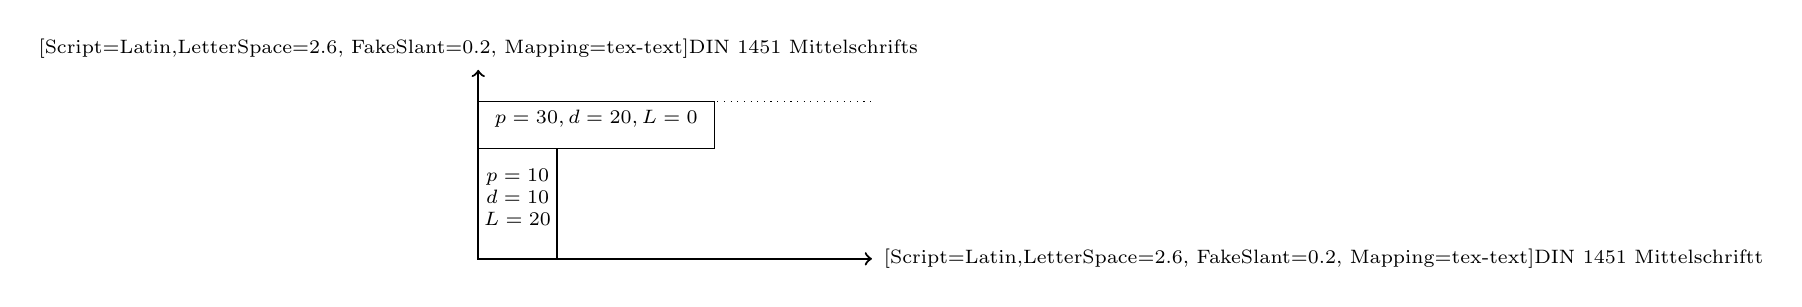
\begin{tikzpicture}[scale=0.2, font=\scriptsize]

      \draw [<->,thick] (0,12) node (yaxis) [above] {\sansitalicfont s}
        |- (25,0) node (xaxis) [right] {\sansitalicfont t};
      \draw[dotted] (0,10) -- (25,10);
        \draw (0,0) rectangle (5,7) node[fn] {$p = 10$\\$d = 10$\\$L = 20$};
        \draw (0,7) rectangle (15, 10) node[fn] {$p = 30, d=20, L=0$};
    
    \end{tikzpicture}
  \end{subfigure}
\caption{Overzealous batch elimination can increase $\Lmax$}\label{fig:bnk1}
\end{figure} %fig:bnk1 (50/10 example)

Unfortunately, we cannot make a general statement that optimal solutions never
have more batches than other feasible solutions -- a simple counterexample is
shown in figure \ref{fig:bnk1}.\footnote{To be more precise, we cannot state
that at least one optimal solution is in the subset of feasible solutions that
uses the fewest number of batches -- a dominance situation that could be
exploited, were it true.}

Starting out with a one-job-per-batch schedule sorted by EDD, we can explore
all feasible batch configurations recursively. To generate any other feasible
schedule (including the optimal solution), jobs $j$ are rescheduled (``moved back'')
from their original batch $k_\text{origin}$ into a prior batch
$k_\text{earlier}$. This eliminates $k_\text{origin}$ and requires, of course,
that $k_\text{earlier}$ has sufficient capacity. If the job's processing time
$p_j$ exceeds that of $k_\text{earlier}$, then the lateness of batches between
$k_\text{earlier}$ and $k_\text{origin}$ will increase; the merit of such a move
cannot be judged in prior, so it is an \textit{unsafe} batch elimination.
\textit{Safe} eliminations, on the other hand, will never worsen $\Lmax$, and
only they can be considered when bounding $n_k$ a priori.

Algorithm \ref{alg:bounding_nk} outlines a recursive method to find an upper
bound on $n_k$, recognizing safe batch eliminations only.

\begin{algorithm}[h]
\fontsize{9pt}{11.5pt}\selectfont
\begin{algorithmic}
\If{no open jobs left} \Comment{if this is a ``leaf node'' in the recursion}
  \State update UB$(n_k)$
\EndIf
\State find the combination of unsafe later jobs that fills up the capacity
most, leaving us with capacity $b_r$ 
\State find all combinations $x$ of safe later jobs that fit into $b_r$
\Repeat
  \State $x$ = next safe job combination
  \State \textit{ignoreJobs} $\gets x$ \Comment{make the moves, let the next recursion
  level deal with the rest of the jobs}
  \State spawn and run child node with $J \setminus$ \textit{ignoreJobs}
  \State \textit{ignoreJobs} $\gets$ \textit{ignoreJobs} $\setminus x$
\Until{all combinations have been explored}
\State return
\end{algorithmic}
\caption{Recursive algorithm to find an upper bound on $n_k$}
\label{alg:bounding_nk}
\end{algorithm}

This algorithm evidently requires exponential time. A relaxed variant is a
possible option: if only a single unsafe move \textit{into} a batch is possible,
no safe eliminations into that batch are considered at all and we skip to the
next batch. This would greatly speed up the recursion but also significantly
weaken the usefulness of the resulting upper bound.

In a brach-and-bound decomposition approach in which batches are modelled
individually, an upper bound on $n_k$ could be used to limit the depth of the
search tree, or, in combination with a method to determine a lower bound on the
remaining jobs' $n_k$ at every node, to actively prune the search tree during
the search. The latter method, however, would also run in exponential time as
it, again, would require knapsack-type reasoning unless we use a much less powerful
relaxation.

\section{CP Model}
\subsection[Constraint on the number of batches with length $P_k >
p$]{Constraint on number of batches with length {\sansitalicfont
P\textsubscript{k}} > {\sansitalicfont p}}

Since \marginpar{\em\small I haven't found an elegant way to turn this into a
gcc constraint, but I also fail to see how it would be useful -- this constraint
matches \textrm{all} feasible solutions, not just a superset of the optimal
one.} batches take on the processing time of their longest job, there is at
least one batch with $P = \underset{j}{\max} p_j $. We can proceed to fill batches with jobs, ordered by non-increasing processing
time, based on algorithm \ref{alg:findBatchlengthCards}. 

\begin{algorithm}[h!]
\fontsize{9pt}{11.5pt}\selectfont \begin{algorithmic} \State $J^{\star} \gets J$
\Comment{initialize all jobs as unassigned jobs} \State $n_k \gets 1$; $S_k
\gets \{0\}$; $P_{k,\text{min}} \gets \{0\}$ \Comment{Create one empty batch of
size and length zero} \State sort $J^{\star}$ by processing time, non-increasing
\Repeat \State $j \gets J^{\star}$.pop() \Comment{select job for assignment,
longest job first} \Loop $\;$ through all $n_k$ existing batches $k$, first
batch first \State $k_p \gets \emptyset$ \Comment{no feasible batch} \State
$c_\text{min} = b$ \Comment{currently known minimum remaining capacity} \If{$s_j
< b-S_k$ and $b-S_k < c_\text{min}$} \State $k_p \gets k_p$; $c_\text{min} \gets
b-S_k$ \EndIf \EndLoop \If{$|k_p| = 1$} \State $S_{k_p} \gets S_{k_p} + s_j$
\Comment{assign job $j$ to batch $k_p$} \Else \If{$n_k < LB(n_k)$} \State $n_k
\gets n_k + 1$\Comment{open new batch} \State $S_{n_k} \gets s_j$;
$P_{n_k,\text{min}} \gets p_j$ \Comment{assign $s_j$ and $p_j$ to the new batch}
\Else \State leave the loop now and end.  \EndIf \EndIf \Until{$J^{\star}$ is
empty} \end{algorithmic} \caption{Generating lower bounds on batch lengths}
\label{alg:findBatchlengthCards} \end{algorithm}
At the end of this algorithm, we can state: \begin{alignat}{2} &
\mathtt{globalCardinality}( |P_{k-1,\text{min}} > P_k \geq P_{k,\text{min}} |
\geq 1) \quad && \forall k \in \{k_0,\dots,k_{LB(n_k)}\} \end{alignat}

The algorithm sorts jobs by non-increasing $p$, and then fills batches job by
job. If a job fits into a previous batch, it is assigned there. If a job fits
into multiple previous batches, it is assigned to the batch with the smallest
remaining capacity. This is called \textit{best-fit decreasing} rule,
and works as follows: let $J^\star$ be the set of jobs sorted by $p$, then at
least one batch will be as long as the longest job $j^\star_1$. If the next $n$
jobs fit into this batch, then there is at least one batch not shorter than
$j^\star_{n+1}$, and similarly for subsequent batches. 

Unfortunately, the optimal solution may perform better than the packing heuristic in
terms of ``vertical'' ($s_j$) bin packing, and may thus require fewer batches.
We therefore need to find a lower bound $LB(n_k)$ on the number of batches, and
we can only guarantee the first $LB(n_k)$ of the above constraints to hold in
the optimal solution. Finding a true lower bound is a two-dimensional bin
packing problem, which runs in exponential time, so we
have to come up with an even lower bound -- right now I can only think of $j_0$,
the number of jobs ordered by decreasing $s_j$ that can never fit into a batch
together.

\subsection[Constraint on the number of batches with due date $D_k >
d$]{Constraint on number of batches with length {\sansitalicfont
D\textsubscript{k}} > {\sansitalicfont d}}

In a similar fashion, we can determine that the second batch must be due no
later than the earliest-due job $j_{m+1}$ that can \textit{not} fit into the first
batch -- if we sort jobs by due date and fit the earliest $m$ jobs into the first
batch -- and so on for subsequent batches. Once again, since best-fit decreasing
may not perform optimally in terms of ``vertical'' packing, this may not be
valid for batches beyond the known $LB(n_k)$.

\subsection[All-different constraints on $P_k$ and $D_k$]{All-different
constraints on {\sansitalicfont P\textsubscript{k}} and {\sansitalicfont
D\textsubscript{k}}}

Furthermore, if all jobs have different processing times, \marginpar{\em\small I haven't found a way to implement this efficiently in CP
Optimizer; I also don't quite see how it would constrain anything.}all batches will have different
processing times as well: \texttt{alldifferent}$(P_k)$. If $m$ out of $n_j$ jobs
have different processing times, we can still enforce
\texttt{k\_alldifferent}$(P_k, m)$. 

Similarly, we knows that the constraint \texttt{k\_alldifferent}$(D_k, m)$ must
be true if $m$ out of $n_j$ jobs have different due dates.
\begin{comment}
\section{Decompositions}
\subsection{Move-back decomposition}
Turn it into a satisfiability problem for $\L_{\text{max,inc}} - 1$.


Another possible way to set up a branch-and-bound search for solutions works as
follows: first, consider all jobs to be assigned to individual batches, i.e.
$B_j = k_j \; \forall j \in J$. Compute the $\Lmax$ for this schedule. Then, at
every level of the search tree, move a job $j$ into any earlier batch $k \leq
k_j$, but only if that move does not violate $k$'s capacity and only if it
improves $\Lmax$. Not moving a job is permissible but no two jobs 
\end{comment}

\section{MIP model II}\label{sec:koschmipmodel}
\begin{model}[h]
\begin{alignat}{2}
\mathrm{Min.}\quad & \Lmax && \\
\mathrm{s.t.}\quad &\sum_{k \in K} x_{jk} = 1 \quad && \forall j \in J \\
  &\sum_{j \in J} s_j x_{jk} \leq b \quad && \forall k \in K\\
  &p_j x_{jk} \leq P_k \quad && \forall j \in J, \forall k \in K\\
  &C_{k-1} + P_{k} = C_k \quad && \forall k \in K\\
  &(d_{max} - d_j)(1 - x_{jk}) + d_j \geq D_k \quad && \forall j \in J, \forall k \in K\\
  &D_{k-1} \leq D_k \quad && \forall k \in K \label{c:malapp-edd} \\
  &C_k - D_k \leq \Lmax \quad && \forall k \in K\\[2ex]
  &C_k \geq 0, P_k \geq 0 \text{ and } D_k \geq 0 \quad && \forall k \in K  
\end{alignat}
\caption{Malapert's original MIP model}
\label{model:malapertmip}
\end{model}


\begin{comment}
\chapter{My solution}
\section{MIP formulation improvements}
\section{CP formulation improvements}

\chapter{Discussion}


\end{comment}
\pagebreak

\bibliographystyle{plainnat}
\bibliography{bibliography}{}
\vskip 4em

\end{document}

